\documentclass[12pt, openany]{amsart}
\usepackage[utf8]{inputenc}
\usepackage[T1]{fontenc}
\usepackage{amsmath,amssymb,amsthm}
\usepackage{pgf,tikz,pgfplots}
\usetikzlibrary{arrows}
\usepackage{color, marginnote}

\begin{document}

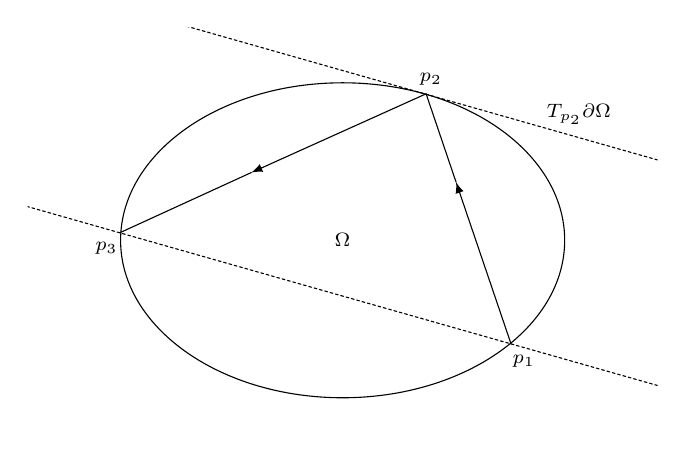
\begin{tikzpicture}[line cap=round,line join=round,>=triangle 45,x=2.0cm,y=2.0cm]
\clip(-2,-1.2) rectangle (2,1.35);
\draw [rotate around={0:(0,0)}] (0,0) ellipse (2.82cm and 2cm);
\draw [dash pattern=on 1pt off 1pt,domain=-3.19:3.33] plot(\x,{(--32-8.43*\x)/29.69});
\draw [dash pattern=on 1pt off 1pt,domain=-3.19:3.33] plot(\x,{(-10.52-8.43*\x)/29.69});
\draw [-latex] (1.07,-0.66) -- (0.72,0.37);
\draw [-latex] (0.53,0.93) -- (-0.58,0.43);
\draw (-0.58,0.43)-- (-1.41,0.05);
\draw (0.72,0.37)-- (0.53,0.93);
\begin{scriptsize}
\draw[color=black] (1.15,-0.77) node {$p_1$};
\draw[color=black] (0.56,1.02) node {$p_2$};
\draw[color=black] (-1.5,-0.05) node {$p_3$};
\draw[color=black] (1.5,0.8) node {$T_{p_2}\partial\Omega$};
\draw[color=black] (0,0) node {$\Omega$};
\end{scriptsize}
\end{tikzpicture}

\end{document}